\documentclass[11pt,letterpaper]{article}
\usepackage[lmargin=1in,rmargin=1in,tmargin=1in,bmargin=1in]{geometry}
\usepackage{../style/homework}
\usepackage{../style/commands}
\setbool{quotetype}{true} % True: Side; False: Under
\setbool{hideans}{true} % Student: True; Instructor: False

% -------------------
% Content
% -------------------
\begin{document}

\homework{13: Due 11/07}{Above all, don't fear difficult moments. The best comes from them.}{Rita Levi-Montalcini}

% Problem 1
\problem{10} Consider the linear function $f(x)= 7 - \frac{6}{7} x$.
	\begin{enumerate}[(a)]
	\item Find the rate of change of $f(x)$.
	\item Is $f(x)$ increasing or decreasing? Explain.
	\item Find the $y$-intercept of $f(x)$.
	\item Find $f(-3)$.
	\end{enumerate}



\newpage



% Problem 2
\problem{10} Using the plot of the linear function $f(x)$ below, answer the following: 
        \begin{enumerate}[(a)]
        \item Find the slope of the given line.
        \item Find the $y$-intercept of the given line.
        \item Find $f(x)$.
        \item Find the $x$-intercept of $f(x)$. 
        \end{enumerate}
	\[
	\fbox{
	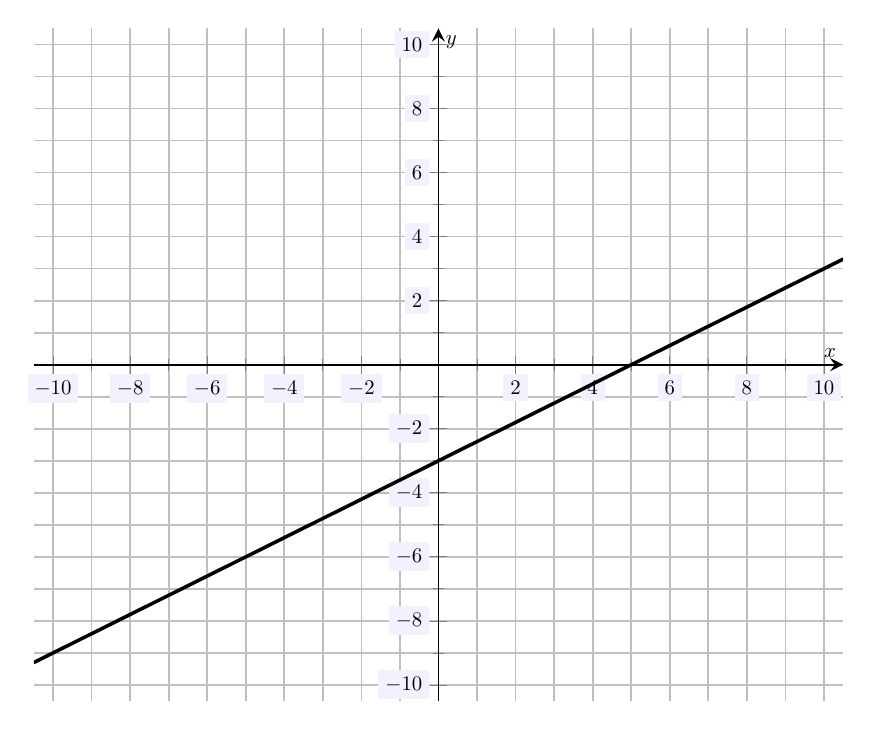
\begin{tikzpicture}[scale=1.5,every node/.style={scale=0.5}]
	\begin{axis}[
	grid=both,
	axis lines=middle,
	ticklabel style={fill=blue!5!white},
	xmin= -10.5, xmax=10.5,
	ymin= -10.5, ymax=10.5,
	xtick={-10,-8,-6,-4,-2,0,2,4,6,8,10},
	ytick={-10,-8,-6,-4,-2,0,2,4,6,8,10},
	minor tick = {-10,-9,...,10},
	xlabel=\(x\),ylabel=\(y\),
	]
	\addplot[domain=-10.5:10.5,samples=2,line width=0.03cm] (x, 3/5*x - 3);
	\end{axis}
	\end{tikzpicture}
	}
	\]


\end{document}